% filepath: PID-in-Modern-Cherenkov/Sections/photomultipliers/pmts.tex
% Content for the "PMTs" subsection

\subsection{PMTs}

Photomultiplier tubes (PMTs) are photon sensitive detectors. A photon incident on a photocathode releases an electron through the photoelectric effect. These detectors then multiply the current from the electron by large amounts through emission of secondary electrons at the dynodes. This enables individual photons to be detected even when the incident flux of photons is low.

\begin{figure}[h]
\centering
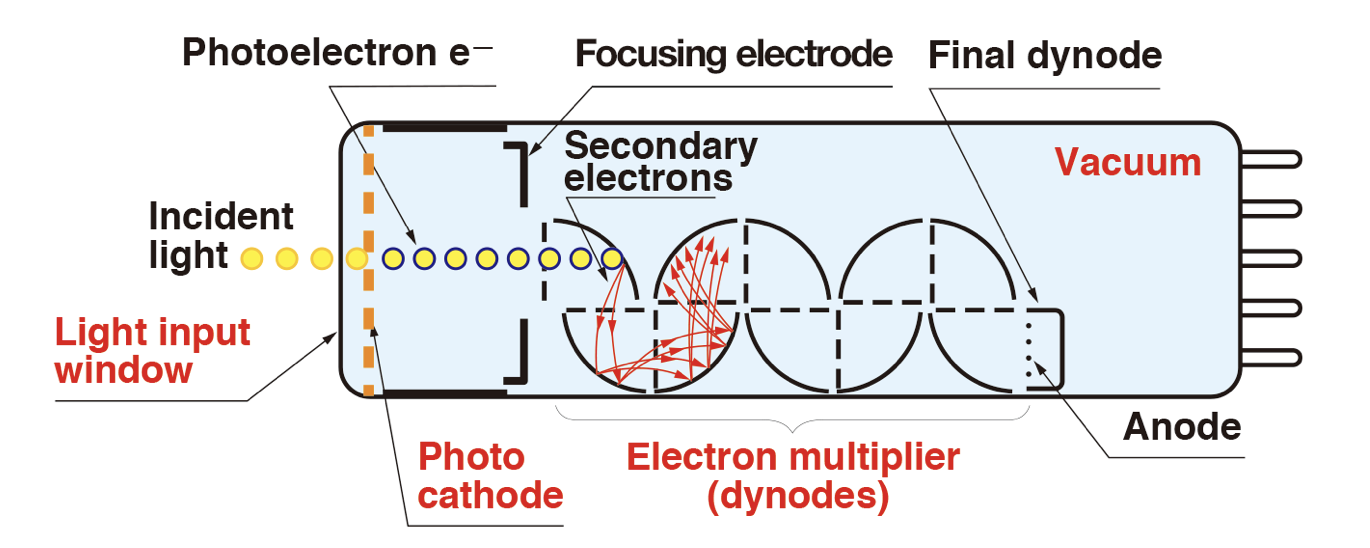
\includegraphics[width=\linewidth]{Images/pmt.png}\label{fig:traditional-pmt}
\end{figure}

The best modern photocathodes used in Cherenkov imaging applications typically have a quantum efficiency (QE) of up to ~30\%, meaning that only 30\% of incident photons satisfy the work function and produce a photoelectron\cite{average-QE-pmts_2018} that reaches the dynodes. The QE of a photocathode is wavelength dependent. For applications in imaging Cherenkov photons, a peak QE around the blue wavelengths is most desirable.

The gain of a PMT is the factor the photoelectron current is increased by at the anode. Modern technologies are able to achieve a gain of up to ~\(10^8\), allowing individual photons to be easily detected. Optimising the dynode voltage, geometry and material are all factors that contribute to higher gain.

PMTs are simple and versatile devices that are still employed in many applications today, including Cherenkov imaging. However, due to the distance between dynodes, they are sensitive to magnetic fields. Since many detector systems at research facilities employ the use of solenoids for various experiments, they are often unfeasible. The solution is to significantly restrict the space between the dynodes.